\documentclass[a4paper,12pt]{article}

\usepackage[utf8]{inputenc}
\usepackage{graphicx}
\usepackage{amsmath}
\usepackage{multicol}
\usepackage{breqn}
\usepackage{xcolor}
\newcommand\tab[1][1cm]{\hspace*{#1}}
\definecolor{gray0}{RGB}{235,235,235}
\definecolor{gray1}{RGB}{220,220,220}
\definecolor{gray2}{RGB}{205,205,205}

\begin{document}

	\title{\textbf{Compte rendu Projet 2 - SE201}}
	\date{October 7, 2016}
	\author{Sevin Adrien, Gaillard Vincent, Bias Steven}
	\maketitle

	\Large{\textbf{3 - Pipelining}}\\\break
	\small

	\underline{3.1}\\
		\setlength{\parindent}{5ex}\par
		En observant les instructions, on remarque un data hazard lors de l'execution de l'instruction 3.
		En effet, le store (instrution 3) nécessite la valeur du registre 29, mais celle-ci n'est pas encore à jour.
		L'instruction précédent qui écrit dans ce registre n'est pas encore terminée.\\
		Au cycle 17, la valeur de r29 n'est pas à jour mais elle devrait être chargée par le store qui est en ID.
		Au cycle 18, l'instruction 3 passe directement à l'execution sans avoir attentdu de pouvoir lire la valeur du registre 29.
		Il y a donc bien forwarding.
		\begin{center}
			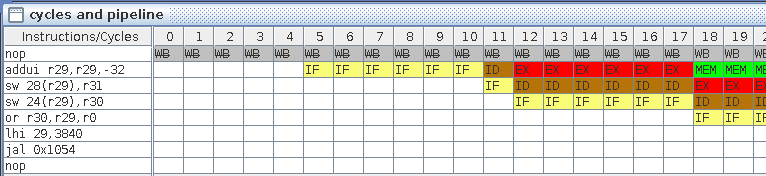
\includegraphics[width=\linewidth]{img/1}
		\end{center}

	\underline{3.2}\\
		\par
		Premier exemple :
		\begin{center}
			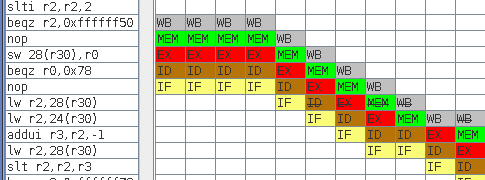
\includegraphics[width=\linewidth * 2 / 3]{img/2}
		\end{center}
		Dans le cas d'une condition (beqz, bnez) à cause d'une "misprediction" le processeur va "flush" les instructions qui avaient été commencé.
		Celles-ci ne se finiront jamais.\\\break
		Deuxième exemple :
		\begin{center}
			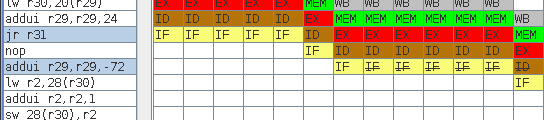
\includegraphics[width=\linewidth * 3 / 4]{img/3}
		\end{center}
		Dans le cas d'un jump (jr) les instructions qui suivent vont être "flushed" et ne seront pas finies.\\

	\underline{3.3}\\
		\par
		Notons que chaque jump et condition est suivie d'une instruction nop. Cette instruction n'est pas "flushed".\\
		Cette technique permet de ne jamais exécuter trop longtemps une instruction qui sera stoppée ensuite.\\
		Concrètement, une instruction "flushed" n'atteind jamais l'état ID.\\

	\break
	\Large{\textbf{4 - Branch Prediction}}\\\break
	\small

	\underline{4.1}\\
		\par
		1-bit saturation counting branch predictor : misprediction rate = 19.14\%\\
		2-bit saturation counting branch predictor : misprediction rate = 18.09\%\\
		Donc le branch predictor sur 2 bits est meilleur que celui sur 1 bit.\\
		On peut aussi voir la meilleure prédiction dans le nombre de "fetches" qui ont due être faits. 2499 contre 2503 pour le \textit{1-bit prediction}.\\
		Cela est due au fait que le \textit{2-bit prediction} permet de supprimer le bruit en quelque sorte.
		Effectivement, si dans un programme il y a beaucoup de boucles (ce qui est le cas ici), même si de temps en temps les boucles seront finies et il y aura une misprediction, on peut supposer que la condition est toujours vérifiée.\\
		Dans ce cas, la méthode \textit{1-bit prediction} entraine deux mispredictions, contre une seule pour celle de textit{2-bit prediction}.\\

	\underline{4.2}\\
		\par
		Selon les branches, on remarque quelques différences entre les \textit{branch predictors}.\\
		Les seules branches où il y a une différences sont :\\
		1-bit saturation counting branch predictor :\\
		bpc: 0x00001104 [4] a:56 t/nt: 10/46 mp/cp: 9/47 mp-ratio: 0,16\\
		bpc: 0x00001158 [88] a:27 t/nt: 21/6 mp/cp: 12/15 mp-ratio: 0,44\\
		2-bit saturation counting branch predictor :\\
		\begin{center}
			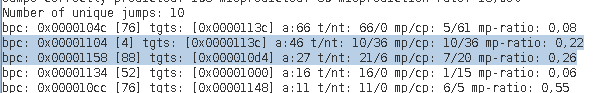
\includegraphics[width=\linewidth]{img/5}
		\end{center}
		On remarque donc que pour la branche [4] le branch predictor sur 1 bit est légèrement meilleur, mais sur la branche [88], le branch predictor sur 2 bit est bien meilleur.\\
		On peut en conclure qu'il est difficile de classer les prédicteurs par performance car elles dépendent du code exécuté.\\

	\underline{4.3}\\
		\par
		\begin{center}
			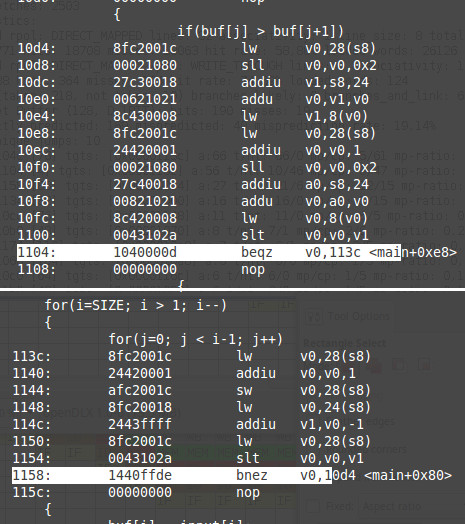
\includegraphics[width=\linewidth / 2]{img/4}
		\end{center}
		La différence à noter est que la branche [4] découle d'une condition (if) alors que la branche [88] découle d'une boucle (for).\\
		Leur comportement est très différent car la condition d'une boucle for n'est fausse que pendant une itération (généralement), ce qui est bien géré par une \textit{2-bit prediction}, alors qu'une condition (if) ne suit pas cette règle.\\
		Ici, la condition fonctionne plutôt par "paquets" de conditions vérifiés/fausses.
		Le \textit{2-bit prediction} prend bien en charge les boucles for mais entraine régulièrement deux misprédictions.\\
		Le \textit{1-bit prediction} est moins intéressante pour les for mais gère mieux les conditions comme décrit juste au dessus.\\

	\underline{4.4}\\
		\par
		Dans le cas où la boucle ou condition de nécessite pas de jump, l'instruction suivante provoque un point (un nop est inséré) de pénalité alors qu'il n'y en a pas dans le cours.\\
		\begin{center}
			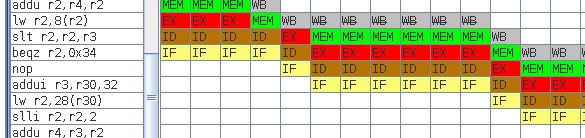
\includegraphics[width=\linewidth * 2 / 3]{img/8}
		\end{center}
		Aussi, si un jump est effectué l'une des deux instructions qui est flushed génère plus de pénalités. C'est une autre différence par rapport au cours.\\
		\begin{center}
			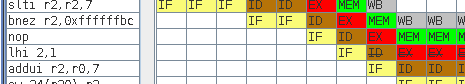
\includegraphics[width=\linewidth * 3 / 5]{img/6}
		\end{center}
		\begin{center}
			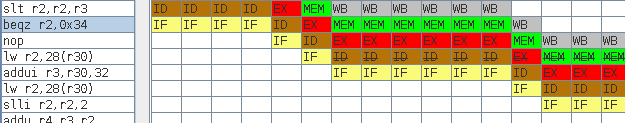
\includegraphics[width=\linewidth * 2 / 3]{img/7}
		\end{center}

	\break
	\Large{\textbf{5 - Data Caches}}\\\break
	\small

	\underline{5.1}\\
		\par
		Nombre de ligne dans le cache : 4
		Taille d'un ligne dans le cache : 4
		Taille totale du cache : 16 octets
			Accesses : 488
			hits : 364
			misses : 124
			hit rate : 74,59%
			loaded words : 124

	\underline{5.2}\\
		\par
		Nombre de ligne dans le cache : 8
		Taille d'un ligne dans le cache : 4
		Taille totale du cache : 32 octets
			Accesses : 613
			hits : 557
			misses : 56
			hit rate : 90,86%
		Nombre de ligne dans le cache : 16
		Taille d'un ligne dans le cache : 4
		Taille totale du cache : 64 octets
			Accesses : 688
			hits : 673
			misses : 15
			hit rate : 97,82%
		Nombre de ligne dans le cache : 32
		Taille d'un ligne dans le cache : 4
		Taille totale du cache : 128 octets
			Accesses : 728
			hits : 721
			misses : 7
			hit rate : 99,04%
		Nombre de ligne dans le cache : 64
		Taille d'un ligne dans le cache : 4
		Taille totale du cache : 256 octets
			Accesses : 728
			hits : 721
			misses : 7
			hit rate : 99,04%
		La taille du cache est égale à le taille d'une ligne multipliée par le nombre de ligne.
		Plus le nombre de ligne augmante, donc la taille du cache augmente, plus le hit rate augmente.
		Les configurations avec 32 lignes et 64 lignes offrent le meilleurs hit rate. Mais on peut dire que la meilleure configuration est celle avec 32 lignes car la taille du cache est plus petite que celle avec 64 lignes.


\end{document}
